\documentclass{beamer}
%
% Choose how your presentation looks.
%
% For more themes, color themes and font themes, see:
% http://deic.uab.es/~iblanes/beamer_gallery/index_by_theme.html
%
\mode<presentation>
{
  \usetheme{default}      % or try Darmstadt, Madrid, Warsaw, ...
  \usecolortheme{default} % or try albatross, beaver, crane, ...
  \usefonttheme{default}  % or try serif, structurebold, ...
  \setbeamertemplate{navigation symbols}{}
  \setbeamertemplate{caption}[numbered]
} 

\usepackage[english]{babel}
\usepackage[utf8]{inputenc}
\usepackage[T1]{fontenc}

\title[Retas e Planos]{Produto Vetorial e Cônicas}
\author{MAP 2110 - Diurno}
\institute{IME USP}
\date{7 de abril}

\begin{document}

\begin{frame}
  \titlepage
\end{frame}

% Uncomment these lines for an automatically generated outline.
%\begin{frame}{Outline}
%  \tableofcontents
%\end{frame}

\section {Produto Vetorial}

\begin{frame}{Definição do Produto Vetorial }
 
 \begin{gather*}
   \vec{a}=(a_1,a_2,a_3)\\
   \vec{b}=(b_1,b_2,b_3)\\
   \vec{a}\times \vec{b}=(a_2b_3-a_3b_2, a_3b_1-a_1b_3, a_1b_2-a_2b_1)
 \end{gather*}

\end{frame}

\begin{frame}{Exemplos}
Uma reta $L$ em $V_2$ contém os pontos $P=(-3,1)$ e $Q=(1,1),$ quais dos seguintes pontos também estão em $L$
\begin{itemize}
   \item[A]$(0, 1, 2) \times (1,0,-1)$
   \item[B]$ (\mathbf{i}\times\mathbf{k})\times\mathbf{j}$
   \item[C]$ (\mathbf{i}\times\mathbf{i})\times\mathbf{j}$
   \item[D]$ (\mathbf{i} + 2\mathbf{j}) \times (2\mathbf{i} - \mathbf{k}$)
\end{itemize}
\end{frame}
\begin{frame}
  

\end{frame}

\begin{frame}{Propriedades}
  \begin{itemize}
    \item $(\vec{a}\times \vec{b}) = - (\vec{b}\times \vec{a})$
    \item $\vec{a}\times(\vec{b} + \vec{c})=\vec{a}\times \vec{b} + \vec{a}\times\vec{c}$
    \item $\alpha(\vec{a}\times \vec{b})=\alpha\vec{a}\times \vec{b}$
    \item $\|\vec{a}\times\vec{b}\|^2 =\|\vec{a}\|^2 \|\vec{b}\|^2 -(\vec{a}\cdot\vec{b})^2$  \end{itemize}

\end{frame}
\begin{frame}
  
\end{frame}


\begin{frame}{Exercício}
  Sejam dados os vetores $\vec{a}=2\mathbf{i}-\mathbf{j}+2\mathbf{k}$ e 
  $\vec{c}=3\mathbf{i} +4\mathbf{j} -\mathbf{k}$, encontrar um vetor $\vec{b}$ tal que
  $\vec{a}\times \vec{b}=\vec{c}.$ Esta solução é única?
\end{frame}

\begin{frame}{solução}
Seja $\vec{b}=b_1\mathbf{i}+b_2\mathbf{j} + b_3\mathbf{k}$
Então podemos escrever usando a propriedade distributiva :
\begin{gather*}
  \vec{a}\times \vec{b}=\vec{a}\times b_1\mathbf{i} + \vec{a}\times b_2\mathbf{j} + 
  \vec{a}\times b_3\mathbf{k}\\
  \text{ usamos que } \mathbf{i}\times\mathbf{j} = \mathbf{k}\text{ } \mathbf{j}\times\mathbf{k} = \mathbf{i}\text{ }
  \mathbf{k}\times\mathbf{i} = \mathbf{j}\\
  \vec{a}\times \vec{b} = (-b_3-2b_2)\mathbf{i} + (2b_1-2b_3)\mathbf{j} +(b_1 +2b_2)\mathbf{k} \\
\end{gather*}
\end{frame}

\begin{frame}
  Comparando os vetores temos o sistema
  \begin{gather*}
    -2b_2 - b_3 = 3 \\
    2b_1 - 2b_3 = 4 \\
    b_1 + 2b_2 = -1
  \end{gather*}
  O sistema é indeterminado e podemos escrever as soluções
  como $\vec{b}= (2\mathbf{i} - \frac{3}{2}\mathbf{j}) + b_3(\mathbf{i}-\frac{1}{2}\mathbf{j}
  +\mathbf{k})$

  Para que $\vec{a}\cdot \vec{b}=1$ a solução é única ($b_3=\frac{-11}{9}$)

  
\end{frame}

\section{Cônicas}

\begin{frame}{Definição}
  O Apostol apresenta três possíveis definições de cônicas, e todos são equivalentes.
  Mas vamos usar a definição que faz mais uso do conceito de vetor.Nosso situação agora 
  num plano. Então podemos fazer todas as contas em $V_2$.

  \textbf{Definição:} Se $L$ é uma reta em $V_2$, $F$ é um ponto fora de $L$ e $e>0$ um 
  número real positivo, então o conjunto:
  $$ C=\{X : \|X-F\| = e d(X,L)    \}$$ é uma cônica, e diremos que $C$ é uma elípse se 
  $e<1$, uma parábola se $e=1$ e uma hipérbole se $e>1$

\end{frame}

\begin{frame}{Como expressar $d(X,L)$}
  
  Nosso problema agora é escrever as equações das cônicas de forma mais direta a partir das definições.
 
  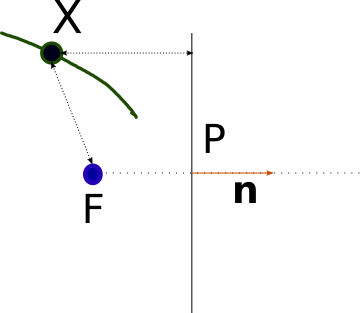
\includegraphics{conica1.png}

\end{frame}

\begin{frame}
Na figura, $\mathbf{n}$ é um vetor unitário apontando para o lado contrário de $F$
Então temos:
\begin{gather*}
  F-P = -d\mathbf{n} \text{ } d>0 \text{ e } F-P = (F-X) + (X-P) \\
  (F-P)\cdot \mathbf{n}= (F-X)\cdot \mathbf{n} + (X-P)\cdot \mathbf{n}\\
  -d = -(X-F)\cdot\mathbf{n} -d(X,L) \implies d(X,L)=|(X-F)\cdot\mathbf{n}-d|
  \end{gather*}
  Isto dá uma forma equivalente de definir a cônica onde não aparece diretamente a reta 
  diretriz!
  $$\|X-F\| = e |(X-F)\cdot\mathbf{n}-d|$$
\end{frame}

    \begin{frame}{Equações polares }
     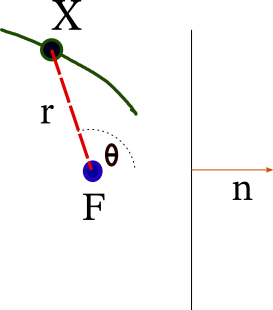
\includegraphics{conica2.png}
    \end{frame}
   
    \begin{frame}{}
     \begin{gather*}
       \|X-F\| = r \text{ } (X-F)\cdot\mathbf{n} = r\cos(\theta)\\
       r= e|r\cos(\theta) - d|
     \end{gather*}
      
    \end{frame}
    \begin{frame}{}
      Se $r\cos(\theta)-d <=0 $ então $|r\cos(\theta)-d |=d -r\cos(\theta)$
      e a equação da cônica fica
      $$ r = \frac{ed}{1+e\cos{\theta}}$$
      No outro caso, se $r\cos(\theta)-d >0$ teremos
      $$ r= \frac{ed}{e\cos{\theta}-1}$$
      claramente isso só ocorre se $e>1$, ou seja,
      só na hipérbole. 
    \end{frame}
\begin{frame}
  
\end{frame}
\begin{frame}{Equações cartesianas} 
  Voltando às equações de definição das cônicas
  $$ \|X-F\| = e |(X-F)\cdot\mathbf{n}-d|$$ 
  Vamos assumir que temos simetria em relação à origem e elevar os lados ao quadrado.
  \begin{gather*}
    (X-F)^2 = e^2((X-F)\cdot\mathbf{n}-d)^2\\
    \|X\|^2 -2X\cdot F + \|F\|^2 = e^2(X.\cdot \mathbf{n})^2 + 2ea(X.\cdot \mathbf{n})
    + a^2\\
    a = ed + e F\cdot\mathbf{n}\\
    \text{ usando a simetria teremos} \\
    \|X\|^2 + e^2a^2 =e^2(X.\cdot \mathbf{n})^2+a^2
  \end{gather*}
\end{frame}

\begin{frame}{Exercício 1}
   fazer o esboço da curva:
   \begin{gather*}
     r= \frac{2}{1+\cos{\theta}} \\
     r = \frac{3}{1+0.5\cos(\theta)}
   \end{gather*}
  
\end{frame}
\begin{frame}
  No primeiro caso temos uma paràbola ($e=1$), com $d=2$, e no segundo caso uma elipse ($e=0.5$)
  com $d=6$
  
\end{frame}





\begin{frame}
  Achar a equação polar da cônica com $e=1/2$ e diretriz $3x+4y=25.$ (Foco em $(0,0)$)
  
\end{frame}

\begin{frame}
  A reta diretriz passa por $(3,4)$, e também $(3,4)$ é um vetor normal à diretriz. Temos então que
  $d=5 =\|(3,4)\|$ como $e=0.5$ a equação polar fica
  $$ r = \frac{2.5}{1+0.5*\cos(\theta-\theta_0)}$$

  
\end{frame}
A reta diretriz passa por $(3,4)$, e também $(3,4)$ é um vetor normal à diretriz. Temos então que
$d=5 =\|(3,4)\|$ como $e=0.5$ a equação polar fica
$$ r = \frac{2.5}{1+0.5*\cos(\theta-\theta_0)}$$
Aqui $\theta_0$ é o ângulo que a reta normal à diretriz forma com $\mathbf{i}$, ou seja 
$\cos(\theta_0)=3/5.$


\end{document}
